
\subsection{Online Tensor Decomposition}
Since dynamic tensor decomposition pursues shorter time factor updates, fast decomposition process results low accuracy factorization when real-time data incomes.

\begin{center}
	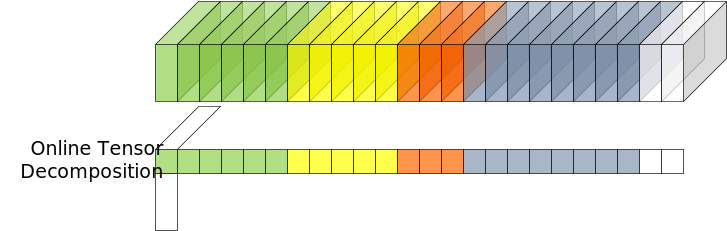
\includegraphics[width=0.8\textwidth]{FIG/0-online-tensor-decomposition.pdf}
\end{center}

\subsubsection{\em Transformed Online CP}
We've developed \tocp by extending the basic intuition of \ocp. To optimize the speed accuracy problem, \tocp resembles \cpals by iteratively updating the factor matrix of temporal mode. In spite of time consumption, however it achieves remarkable accuracy improvement.

\subsubsection{\em DTD}
temporally growing dtd mentioned in Multi-aspect tensor completion

\newpage
\subsection{Drastic Data Handling}
When we decompose a tensor, we can find error norm comparing real and estimated entries. As the tensor temporally grows, we can calculate local and global error norm by measuring incoming slices and the whole tensor respectively.

Drastic data can be detected by measuring local error norm and distribution of previous norms. Using Welford's algorithm, we can track mean and deviation and find out anomalies in current local error norm by z-score calculation. Differentiating the upper and lower limit of z-score, we can trigger one of accuracy optimizing processes. Trigger function now decides whether to split or to concatenate behind after one temporal factor update. It allows to store the tensor efficiently by grouping tensors with similar themes and splitting them otherwise.

\begin{center}
	\includegraphics[width=0.8\textwidth]{FIG/0-drastic-data-handling.pdf}
\end{center}

\subsubsection{\em Split Process}
Anomaly detection in image error norm tells us sudden change in data. What if the incoming data may have a new theme unseen before? It implies that new decomposition starting point with tensor split is needed. In this process, we'd like to apply upper limit ${ul}$ to trigger splitting the tensor into serial tensors of different themes.

\subsubsection{\em Refinement Process}
Refinement process is to concatenate incoming tensor slices whose theme is similar to the previous tensor. Exceedance of lower limit ${ll}$ trigger forgetting preious decomposition result and decompose the tensor once again.

\begin{center}
	\includegraphics[width=0.49\textwidth]{FIG/1-online-tensor-decomposition.pdf}
	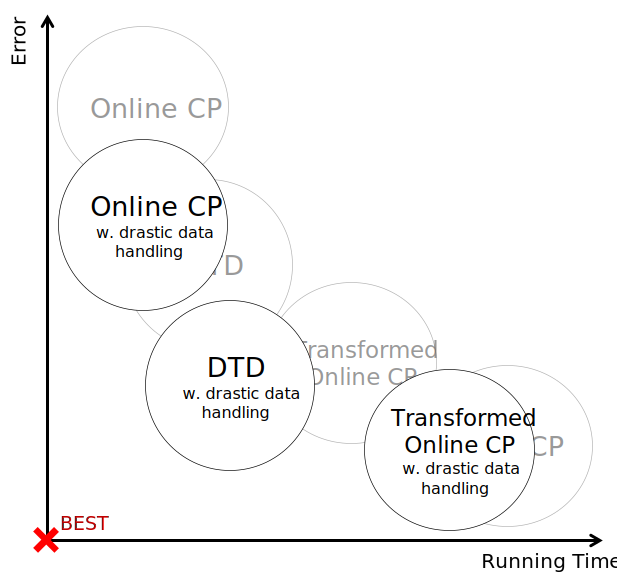
\includegraphics[width=0.49\textwidth]{FIG/1-drastic-data-handling.pdf}
\end{center}
